\documentclass[journal,comsoc]{IEEEtran}
\usepackage[T1]{fontenc}% optional T1 font encoding

\usepackage{ifpdf}
\usepackage{cite}
\ifCLASSINFOpdf
  \usepackage[pdftex]{graphicx}
\else
  \usepackage[dvips]{graphicx}
\fi
\usepackage{amsmath}
\interdisplaylinepenalty=2500
\usepackage[cmintegrals]{newtxmath}
\usepackage{bm}
\usepackage{algorithmic}
\usepackage{array}
\ifCLASSOPTIONcompsoc
  \usepackage[caption=false,font=normalsize,labelfont=sf,textfont=sf]{subfig}
\else
  \usepackage[caption=false,font=footnotesize]{subfig}
\fi
%\usepackage{fixltx2e}
%\usepackage{stfloats}
\ifCLASSOPTIONcaptionsoff
  \usepackage[nomarkers]{endfloat}
 \let\MYoriglatexcaption\caption
 \renewcommand{\caption}[2][\relax]{\MYoriglatexcaption[#2]{#2}}
\fi
\usepackage{url}
\usepackage{hyperref}
\usepackage{bbm}
% correct bad hyphenation here
\hyphenation{op-tical net-works semi-conduc-tor}


\begin{document}
\title{Mixture of Spatial-and-Temporal Network for Hand Pose Estimation}

\author{{Anonymous}% <-this % stops a space
\thanks{Anonymous}}

% The paper headers
\markboth{Journal of \LaTeX\ Class Files,~Vol.~14, No.~8, August~2015}%
{Shell \MakeLowercase{\textit{et al.}}: Bare Demo of IEEEtran.cls for IEEE Communications Society Journals}

% make the title area
\maketitle

\begin{abstract}
As an essential and challenge problem in computer vision, hand pose estimation aims to estimate the hand joint locations. Current hand pose
estimation methods concentrate on the spatial structure of human hand but omit the temporal coherence of consecutive frames.
Motivated by this observation, we present a hand pose estimation method called Mixture of Spatial-and-Temporal Network (\textbf{MSTN})
by keeping a watchful eye on accuracy, efficiency, robustness and stability. We extract the temporal coherence via a set of long-short
term memory (LSTM) nodes and the spatial information by a Deeply-fusion framework simultaneously, then predict the hand pose via spatial
and temporal features. In a nutshell, our proposed \textbf{MSTN} is capable of make use of correlation between images as well as spatial
information. Our method is examined on two publicly available datasets, the experiments demonstrate that our proposed approach achieves
comparable performance with state-of-art methods and runs in real-time (around 75 fps).

\end{abstract}
% Note that keywords are not normally used for peerreview papers.
\begin{IEEEkeywords}
Hand pose estimation, LSTM, Mixture of Experts, Deeply-Fusion.
\end{IEEEkeywords}


% For peer review papers, you can put extra information on the cover
% page as needed:
\ifCLASSOPTIONpeerreview
\begin{center} \bfseries EDICS Category: 3-BBND \end{center}
\fi
%
% For peerreview papers, this IEEEtran command inserts a page break and
% creates the second title. It will be ignored for other modes.
\IEEEpeerreviewmaketitle


\section{Introduction}\label{sec:introduction}
\IEEEPARstart{H}{and} pose estimation is an essential problem in computer vision, and plays an pivotal
role in vision application such as human-computer interface (HCI), augmentation reality (AR)~\cite{barsoum2016articulated}. So
far, there are a plenty of researches on this topic~\cite{guo2017region, quach2016depth, ge2017_3D,
wan2017crossing}, and major progresses have been made thanks to the improvement in deep learning
and low cost depth sensors. Nevertheless, hand is the most complex human part to analyse, and the
problem is still far from solved, it is still difficult to estimate hand pose in the practical scene
owing to several reasons: (1) the image quality is poor because of the commercial depth sensor, (2)
hand is a articulated object with high degrees of freedom (DoFs), the fingers are similar with each
other and apt to occlude each other, (3) in a real scenario, the application must process the depth
image real-timely, which increase the difficulty for estimation.

In general, the purpose of hand pose estimation is to estimate the 3D location of joints. Most existing
methods concentrate on the hand spatial structure modelling, such as the nodes in regression decision
forest and separated stages in cascaded CNN, while ignoring the coherence between the current frame and
the previous frame. For instance, when we humans find the joint locations, we usually search in the
patches around the previous frame's joints. It reveals that the previous frame's pose provides abundant
information for pose estimation. However, many existing methods~\cite{oberweger2015hands, ge2017_3D} learn
the mapping from depth image or 3D volumetric representation to the hand pose. Some methods
~\cite{sun2015cascaded, ye2016spatial} explicitly model the hierarchical hand structure in addition. In
practice, depth images are in selected from videos, and video has time-varying dynamic properties.

\begin{figure*}[t]
    \centering
    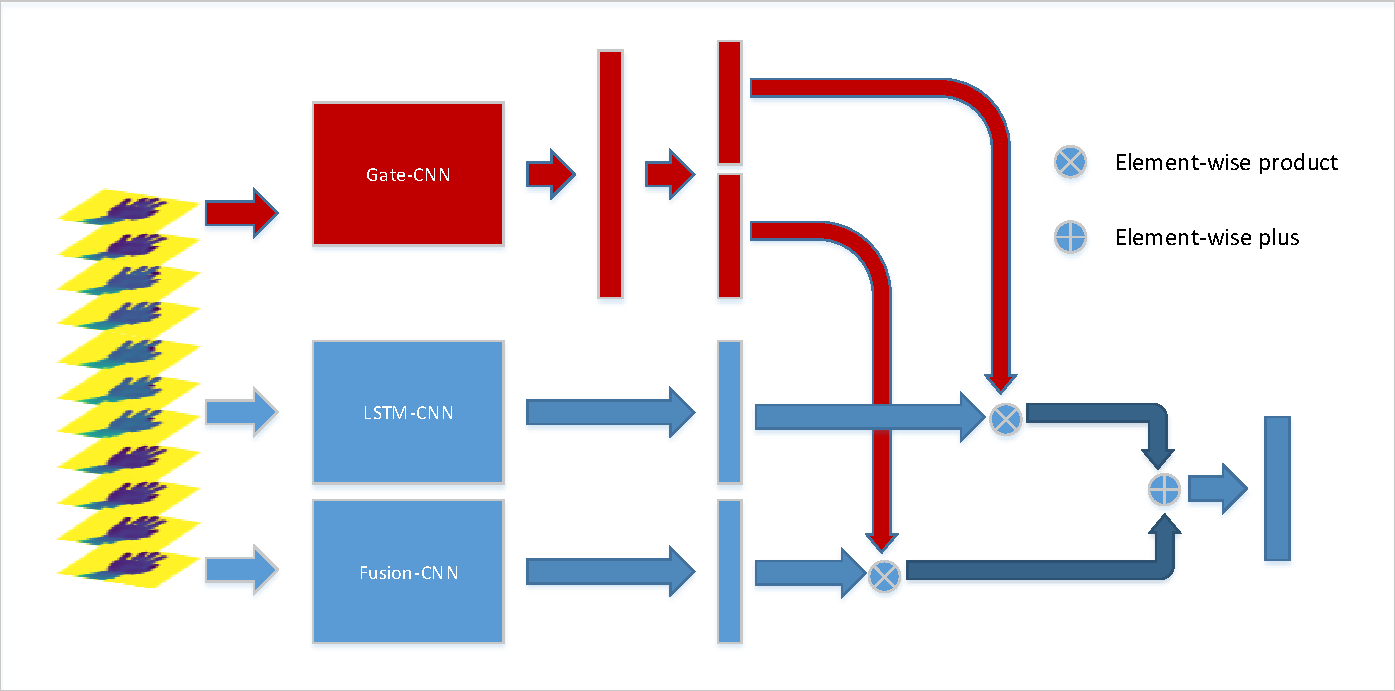
\includegraphics[width=1\linewidth]{src/network/architecture.pdf}
    \caption{The overview of total network. The network is composed of three parts: \emph{Temporal Network}, 
    \emph{Spatial Network} and \emph{Gate Network}. \emph{Temporal Network} extract the correlated features 
    considering the sequentiality of input images via LSTM and \emph{Spatial Network} employ the Deeply-Fusion 
    framework to fuse depth image and sliced 3D volumetric representations, \emph{Gate Network} weights the 
    prediction from each expert and get the final prediction.}
\label{fig:architecture}
\end{figure*}

Motivated by the observation above, we propose a method focus on the spatial structure as well as
temporal information. The different viewpoint for solving the problem is modelled as different part in
our method. Figure~\ref{fig:architecture} shows a holistic illustration for our approach. The first
part is denoted as \emph{Spatial Network} in this paper, which learns the mapping to hand pose from
spatial information. \emph{Spatial Network} works on a single depth image, with the depth image and
corresponding sliced 3D volumetric representation input into the network, spatial information extracted
hierarchically improve the performance of pose estimation. The second part is denoted as \emph{Temporal Network}.
The conventional works~\cite{tang2014latent, zhou2016model, tang2015opening} lay emphasis on the
hierarchical structure or spatial constraint of hand, while ignore the relationship
of the between frames. Motivated by this, we create this network pay attention to the time coherence property
in depth map video. The network take the previous features into account when estimating the pose in current frame,
in other words, the history is memorized by the network and affects the current prediction.

For the sake of accurately estimating the hand pose, we ensemble the aforementioned two networks as an
integration by Mixture of Experts~\cite{jacobs1991adaptive}. The networks for prediction task are called
\emph{experts}, and via \emph{gater} to output a set of weights, the final prediction is obtained by the
weighted combination of the experts outputs. By means of this ensemble approach, spatial information and temporal
coherence are thought to have in mind as a unified scheme. Moreover, the estimation network is evaluated on
two public datasets. Due to the practicability and efficiency, the network could run in real-time on the GPU and achieve
the comparable or better results than state-of-art methods. We summary our contribution in the following two folds:
\begin{itemize}
  \item
  We integrate features from depth map and sliced 3D volumetric representation for hand pose
  estimation by deep fusion network. The experiment reveals that 3D volumetric representation
  benefits the hand pose estimation. Furthermore, we model the coherence among frames by LSTM,
  and implement a hand pose estimation system named \textbf{MSTN} (\textbf{M}ixture of
  \textbf{S}patial-and-\textbf{T}emporal \textbf{N}etwork) with an eye to accuracy, efficiency,
  robustness and stability simultaneously.
  \item
  Our proposed method could run about 75 fps on a single GPU, which meet the real-time demand
  in hand pose estimation. Moreover, we evaluate our approach on two public datasets (e.g. NYU
  and ICVL), and get the comparable or better results than state-of-art methods.
\end{itemize}

% needed in second column of first page if using \IEEEpubid
%\IEEEpubidadjcol

%-------------------------------------------------------------------------
\section{Related Work}\label{sec:related work}
\subsection{Hand Pose Estimation}
The approaches proposed in this area fall in three categories: data-driven, model-based and hybrid approaches.

Model-based approaches commonly evaluate the manually designed energy function on the basis of hand skeleton model,
the problem is formulated as an optimization problem that the objective function measure the discrepancy between
model hypothesis and the actual ones. Oikonomidis et.al ~\cite{oikonomidis2010markerless,oikonomidis2011efficient}
use Particle Swarm Optimization (PSO) solving the optimization problem about the hand model parameters.
With a discriminative initialization method, \cite{tagliasacchi2015robust} employ Iterative Closest Point (ICP)
for optimizing problem. \cite{qian2014realtime} use ICP-PSO for optimization and apply to a sphere-based hand motion model.
\cite{RoditakisMakrisArgyros2017} propose a method that explicitly considers constraints on the 3D locations of fingertips.
Different hand models are adopted in model based methods, such as surface model
~\cite{qian2014realtime,khamis2015learning} and gaussian model~\cite{sridhar2014real,tang2015opening},
etc. While the hand model is intuitive, these methods are sensitive to the initialization, and the errors are accumulated
during the estimation because of the temporal information used.

Data-driven approaches used in hand pose estimation are roughly divided into two camps: randomized decision forest (RDF)
and deep learning based methods. \cite{keskin2012hand,tang2013real,tang2014latent,sun2015cascaded,li20153d} employ RDF
for estimation. Specifically, \cite{keskin2012hand} use RDF-based method for hand part labelling and mean shift algorithm
as the joint finder. \cite{tang2013real} propose a semi-supervised transductive regression forest to label the realistic
dataset and the synthetic dataset, then refine joints by a data-driven, pseudo-kinematic technique. In \cite{tang2014latent},
a latent regression forest is learned for structured hand joints coarse-to-fine search, and \cite{li20153d} integrate
segmentation index points (SIP) achieving a better results. \cite{sun2015cascaded} hierarchically regress the joint
locations with a cascaded scheme. On the other side, CNN based methods learn the mapping from input to the hand pose,
comparing to the RDF based methods, a commonly better result could be achieved because the better features are learned.
Tompson et al.~\cite{tompson2014real} firstly employ CNN in hand pose estimation to regress the heat map and make use
of inverse kinematics algorithm as the post-processing. Oberweger et al.~\cite{oberweger2015hands} use segmented depth
map as input straightly regress 3D joint locations and do joint-specific refinement to increase the accuracy. Then in
~\cite{oberweger2015training}, a feedback loop framework is proposed, which is composed of a predictor for initialization,
a synthesizer for image generation and a updater for refinement. \cite{zhou2016model} design a network embedding the
forward kinematic process, which gets rid of the inconvenient post-processing. \cite{ye2016spatial} presents a method
by applying the kinematic hierarchy to both the input and feature space of the discriminative method and the optimization
of the generative method. Ge et al.~\cite{ge2016robust} predicts the heat-maps by a multi-view regression framework, and
\cite{ge2017_3D} improve this method by applying 3D CNN, which takes multi-view 3D volumetric representations as input for
regressing full 3D hand pose in a single pass. Wan et al.~\cite{wan2017crossing} use VAE and GAN to learn the manifold of
hand pose, with an alignment operation, pose space are projected into a corresponding depth map space via a shared latent
space.

Hybrid approaches\cite{keskin2013real, sharp2015accurate,madadi2017occlusion} retain the advantages of both data-driven and
model-based methods. \cite{keskin2013real} use the hand model for synthetic dataset generation followed by an RDF classifier,
then the mean-shift joint finder is adopted for final joint localization. \cite{sharp2015accurate} follows a different pipeline
which comprising hand RoI extraction, reinitialization and model fitting for hand tracking, hand model is used for extraction
and model fitting, the reinitialization step infer the distribution over hand poses via a layered discriminative model. In
\cite{madadi2017occlusion}, hand pose is recovered through a combination of part-based model fitting and data-driven approaches
in a single frame, and refine occluded joints in a sequence.

\subsection{LSTM}
Due to the feedback loop structure in the recurrent neural network (RNN), it possesses powerful 'long-term dependencies'
modeling capability, and is widely used in computer vision tasks. In general, RNN is difficult to train due to the vanishing
gradient and error blow up problems~\cite{graves2012supervised}. To address these problems, plenties of works design the new
structure based on RNN, and RNN with Long-Short Term Memory (LSTM) neurons~\cite{hochreiter1997long,zaremba2014learning} is the
most frequently-used variant. As shown in Figure~\ref{fig:lstm cell}, a LSTM memory block with a single cell is illustrated. 
It contains three gates: the input gate $i$, the forget gate $g$ and the output gate $o$, the memory is manipulated by these gates, 
which could be erased, updated and read.

\begin{figure}[htbp]
\centering
    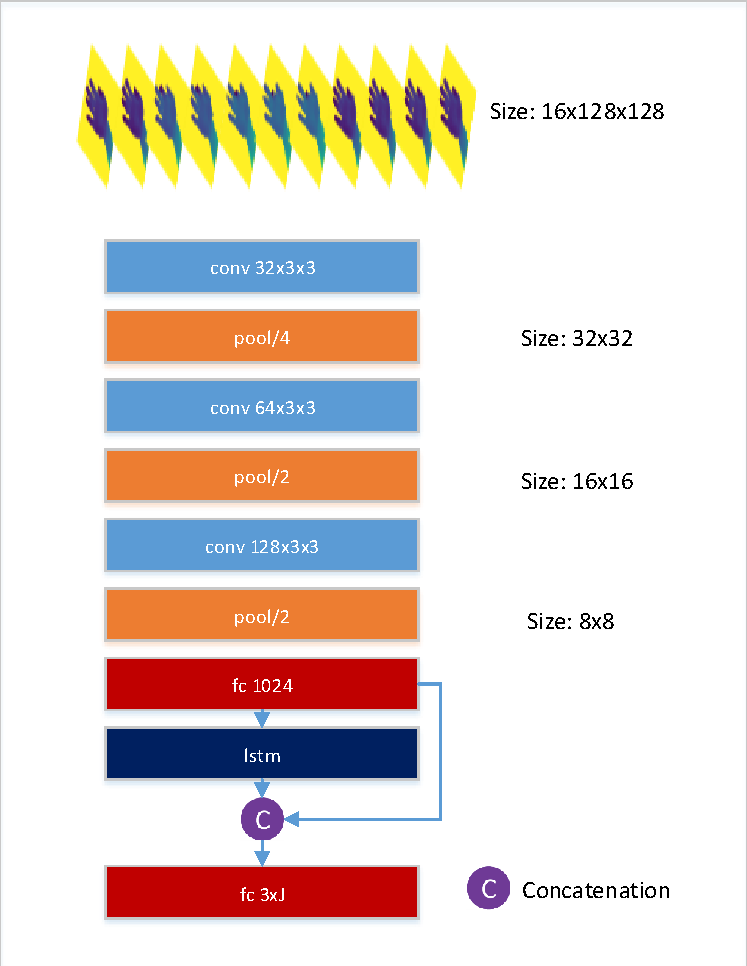
\includegraphics[width=1\linewidth]{src/network/lstm.pdf}
    \caption{Long-Short Term Memory (LSTM) cell. The internal memory is manipulated by several gates.}
    \label{fig:lstm cell}
\end{figure}

Given an input sequence $\mathbf{x} = (x_0, x_1, \dots, x_{T-1})$, the hidden state of LSTM layer $h = (h_0, h_1, \dots, h_{T-1})$ 
and the output $y = (y_0, y_1, \dots, y_{T-1})$ are derived as follows\cite{zaremba2014learning}:
\begin{equation}
\begin{aligned}
&i_t := \sigma(W_{hi} * h_{t-1} + W_{xi} * x_t + b_i) \\
&f_t := \sigma(W_{hf} * h_{t-1} + W_{xf} * x_t + b_f) \\
&o_t := \sigma(W_{ho} * h_{t-1} + W_{xo} * x_t + b_o) \\
&c_t := (f_t \odot c_{t-1}) + (i_t \odot tanh(W_{hc} * h_{t-1} + W_{xc} * x_t + b_c)) \\
&h_t := o_t \odot tanh(c_t)
\end{aligned}
\end{equation}
where $\sigma(\cdot)$ is sigmoid function, $tanh(\cdot)$ is tanh function, $\odot$ is element-wise product, and matrices $W_{h*}, W_{x*}, b_{*}$ ($*$ is in $i, f, o, c$) are shared between cells.

%------------------------------------------------------------------------
\section{Hand Pose Estimation}\label{sec:hand pose estimation}
In this section, we introduce our contributions to hand pose estimation.

\subsection{Problem Analysis}\label{sec:problem analysis}
% prepare the notation for problem
Our objective is to predict the hand joint locations in 3D space from a sequence of depth images,
the locations are represented as a set of keypoints. We denote a single depth image as $\mathit{I}$, and
the corresponding hand pose is
$\mathit{J}=\{\mathit{j}_i\}_i^K \in \mathbb{R}^{3 \times K}$ with $\mathit{j}_i=(x_i,y_i,z_i)$
represents the 3D position of $i$-th joint in the depth image $\mathit{I}$, $K$ is the number of joints,
it is different among datasets.

In this paper, we concentrate on the efficient 3D hand pose estimation from the depth images and
introduce a robust spatial-temporal hand pose estimation approach. In the natural scene, the camera
capture the consecutive frames and hand is contained in the frame.
The hand pose in the between frames is highly correlated. Inspired by the hand pose
tracking~\cite{quach2016depth}, we embed Long Short Time Memory (LSTM) into \emph{Temporal Network}
to extract features consider the sequentiality. Recurrent LSTM encode the original sequential
features into a correlated features for estimation. Furthermore, the spatial information of hand is
important, many approaches focus on tree structured skeleton of hand to address this problem (e.g.
~\cite{li20153d, wan2016direction, ye2016spatial}). And 3D volumetric representation could well reserve
the spatial information~\cite{deng2017hand3d} for solving pose estimation in 3D. We employ the
Deeply-Fusion framework ~\cite{wang2016deeply} to fuse the features from depth image and sliced 3D
volumetric representations, which is called \emph{Spatial Network}. \emph{Temporal Network} and
\emph{Spatial Network} predict hand joint locations based on different features, which plays a
role of experts in the Mixture of Experts (MoE). In MoE, the different experts give out their
predictions and \emph{Gate Network} weights the predictions.

We introduce our method for hand pose estimation step by step. \emph{Basic Network} is introduced
in Section~\ref{sec:basic network}. The \emph{Temporal Network} and \emph{Spatial Network} we
employed are discussed in Section~\ref{sec:temporal netowork} and Section~\ref{sec:spatial network}, and \emph{Gate Network} is
discussed in Section~\ref{sec:gate network}.


% Figure ~\ref{fig:architecture} shows the entire architecture. Aspired by Mixture of Experts
% ~\cite{jacobs1991adaptive}, network is composed of two parts: \emph{Gate Network} and
% \emph{Expert Networks}, we use a \emph{Gate Network} to control two expert networks.
% Each expert predicts the 3D pose given the input image, the \emph{Gate Network} weights
% the prediction from each expert. The experts concentrate on different information.
% \emph{Temporal Network} takes temporal context into account between the consecutive frames.
% \emph{Spatial Network}, thinking over spatial information, fuses the features from depth
% map and 3D volumetric representation.

\subsection{Basic Network}\label{sec:basic network}
We first propose \emph{Basic Network} as the basic network for estimation. As shown in Figure
~\ref{fig:basic network}, the \emph{Basic Network} is a typical CNN architecture, which is composed
of several stacked convolution layers, with max-pooling layer do downsampling operation in between
them. The fully connected layers perform as a regressor for last regression. In addition, the activation
function used in network is ReLU, which provides non linear ability and improves the robustness. To resist
overfitting, the Dropout is adopted in fully connected layers.

The \emph{Basic Network} performs a pre-trained network for \emph{Temporal Network}, and it could get a
satisfied result as shown in the experiments.

\subsection{Temporal Network}\label{sec:temporal netowork}
\begin{figure}[t]
    \centering
    \subfloat[Basic Network]{
        \label{fig:basic network}
        \begin{minipage}[t]{116pt}
            \centering
            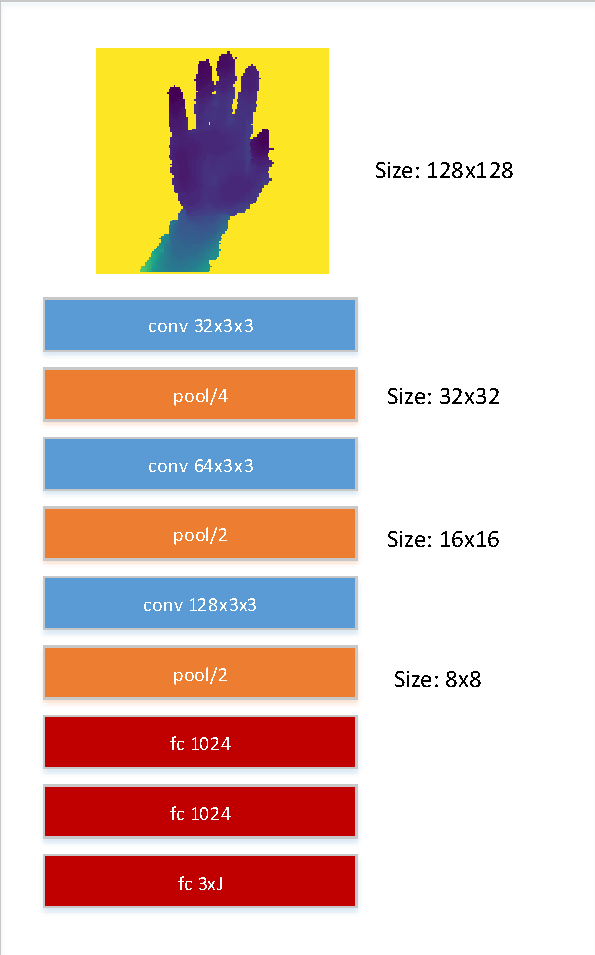
\includegraphics[width=1\linewidth]{src/network/baseline.pdf}
        \end{minipage}
    }
    \subfloat[Temporal Network]{
        \label{fig:temporal network}
        \begin{minipage}[t]{116pt}
            \includegraphics[width=1\linewidth]{src/network/temporal.pdf}
        \end{minipage}
    }
\caption{\emph{Basic Network} and \emph{Temporal Network}. In \emph{Basic Network}, convolution
layers and fully connected layers are followed by activation function is ReLU, and dropout is
adopted to resist overfitting. In \emph{Temporal Network}, the parameters in previous layers are
borrowed from \emph{Basic Network}, LSTM layer and last fully connected layer are trained when
the input is a sequence of images.}
\label{fig:basic and lstm network}
\end{figure}

As we know, the hand poses between successive frames are correlated (e.g. when grabbing, the joints
on fingers are most likely to be closer). Currently, an Recurrent Neural Network (RNN) with Long
Short-Term Memory (LSTM) units~\cite{zaremba2014learning} is widely used because they are expressive
and easy to train. The LSTM network is mostly used for modeling the long term temporal correspondence.
\cite{quach2016depth} use RNN regress the joint location straight forward, and training CNN and RNN
simultaneously. We do several modifications to extract robust features and have better result with
temporal information.

As is shown in Figure~\ref{fig:temporal network}, a sequence of depth images $\{I_1, I_2, \dots, I_N\}$ is
taken as input and the network gives out the estimated pose. Think about the $t$-th depth image $I_t$,
the image flow through the convolution network and the feature extracted is denoted as follows,
\begin{equation}
\phi(I_t)=f_{\theta_c}(pre(I_t))
\end{equation}
where $f_{\theta_c}(\cdot)$ is a convolutional network with parameters $\theta_c$ and
$pre(\cdot)$ is the preprocessing to crop out the hand. The preprocessing step is declared
in Section.~\ref{sec:experiments}. The features are fed into LSTM and LSTM layer outputs its hidden
state,
\begin{equation}
h_t=f_{\theta_l}(h_{t-1}, \phi(I_t))
\end{equation}
where $f_{\theta_l}$ is the parameters in LSTM cell. The new features and original features
are concatenated then fed into the last fully connected layer and network give out the predictions.

In the training stage, the parameters of layers before LSTM layer are borrowed from \emph{Basic Network}
and fixed, then we train LSTM and last fully connected layer solely.

\subsection{Spatial Network}\label{sec:spatial network}
According to the discussion in \cite{supancic2015depth, deng2017hand3d, ge2017_3D}, 3D
volumetric representation benefits the hand pose estimation. However, due to the high
cost of 3D convolution, the input is mostly small such as $32 \times 32 \times 32$ in
~\cite{deng2017hand3d, ge2017_3D}, it sacrifices the detail of depth image. We employ
an eclectic solution, the background is omitted in our 3D representation, and the space
is sliced into 8 pieces to preserve more details. The exemplar is shown in Figure
~\ref{fig:spatial network}.

The sliced 3D volumetric representation keeps the structure of hand, we can clearly find all
finger tips in the first layer, with a low cost for memory at the mean time. Nevertheless,
the depth information is deprecated in our sliced 3D volumetric representation, it makes harder
to estimate the hand joint locations. To obtain the hand structure and depth
information simultaneously, we input depth image and 3D volumetric representation at the
same time. In Figure~\ref{fig:spatial network}, we employ Deep-Fusion
framework~\cite{Chen_2017_CVPR} to fuse the features and the network is named as \emph{Spatial Network}.
The left part is same as \emph{Basic Network}, and the right part is similar with the left part.

In \emph{Spatial Network}, the different features are fused together hierarchically.
which could be expressed as:
\begin{equation}\label{eq:deep fusion}
\begin{aligned}
&f_0 = f_{depth} \oplus f_{3D} \\
&f_l = \mathbf{H}_l^{depth}(f_{l-1}) \oplus \mathbf{H}_l^{3D}(f_{l-1}) \\
&\forall l=1, \dots , L
\vspace{1em}
\end{aligned}
\end{equation}
The $\oplus$ is element-wise mean, $f_{depth}$ and $f_{3D}$ are the features output from
two pooling layers, $\mathbf{H}$ is the transformation for features,
$l$ is the index for layer.

Owing to the several fully connected layers, the network tends to overfitting, so we use
an auxiliary loss as the regularization as well as dropout. In Figure~\ref{fig:spatial network},
every fully connected layer is followed by a dropout layer, the nodes are dropout randomly
with 30\% probability. For the purpose of obtaining more representative capability for each input,
the auxiliary paths are added in training stage. As shown in the green boxes, the layers in the
auxiliary paths are same as the main network, the layers connected by the blue dotted line
share parameters. And in the training stage, the total losses are consist of three losses,
i.e. three regression loss in auxiliary paths and main network. When testing, the auxiliary
pathes are removed.
\begin{figure*}[t]
    \centering
    \includegraphics[width=0.5\linewidth]{src/network/spatial.pdf}
    \caption{\emph{Spatial Network}. Depth image and sliced 3D volumetric representation are input
    into \emph{Spatial Network}, the different features are fused together hierarchically. For the
    purpose of obtaining more representative capability for each input, the auxiliary paths are added
    in training stage, and the layers in the auxiliary paths are same as the main network. In the training
    stage, the total losses are consist of three losses, i.e. three regression loss in auxiliary paths
    and main network. When testing, the auxiliary pathes are removed.}
\label{fig:spatial network}
\end{figure*}

\subsection{Gate Network}\label{sec:gate network}
\begin{figure}[t]\footnotesize
\centering
    \includegraphics[width=1\linewidth]{src/network/gate.pdf}
    \caption{\emph{Gate Network}, the network outputs weights for two predictions from \emph{Spatial Network} and \emph{Temporal Network}.
    Because the dimension of output is twice as much as the prediction, we double the kernel size compare with \emph{Basic Network}.}
\label{fig:gate}
\end{figure}
The foregoing \emph{Temporal Network} and \emph{Spatial Network} stand in the different views
for estimating the joints, we name the predictions as $\mathit{J}_{temp}$ and $\mathit{J}_{spa}$. To improve
the performance, we ensemble them via Mixture of Experts (MoE)~\cite{jacobs1991adaptive}, by adaptively integrating
different regressors for the last prediction.

\emph{Gate Network} weights two predictors, and give out the last prediction according to
the weights of predictions as follow:
\begin{equation}\label{eq:gate network}
\centering
\mathit{J}_{out} = \mathit{g}_1 \mathit{J}_{temp} + \mathit{g}_2 \mathit{J}_{spa}
\end{equation}
where $\mathit{g}_1$ and $\mathit{g}_2$ are the weight of \emph{Gate Network} and $\mathit{g}_1, \mathit{g}_2 \in
\mathbb{R}^{3 \times K}$. The final prediction $\mathit{J}_{out}$ is estimated as the weighted sum of each prediction.

Because \emph{Temporal Network} considers the temporal information and \emph{Spatial Network}
extracts the spatial information, mixture of experts infer the hand joint location based on
spatial and temporal features. Comparing with \emph{Basic Network}, \emph{Gate Network} outputs higher
dimension weights, so we employ a more complex network by increasing the number of convolution kernels.
Specifically, we double the parameters in \emph{Gate Network} than \emph{Basic Network}, as shown in Figure~\ref{fig:gate}.

%-------------------------------------------------------------------------
\section{Experiments}\label{sec:experiments}
In this section, we evaluate our approach on two public datasets, NYU~\cite{tompson2014real}
and ICVL~\cite{tang2014latent}, for comparison with the state-of-art methods. In addition, we
do ablation experiments and analyse the performance of each component. We first describe our
experiment setting.

\begin{figure*}[t]\footnotesize
\centering
    \subfloat[]{
        \label{fig:comparison NYU}
        \begin{minipage}[t]{267pt}
            \centering
            \includegraphics[width=1\linewidth]{src/experiment/eval/NYU/comparison/comparison_frameswithin.pdf}
        \end{minipage}
    }
    \subfloat[]{
        \label{fig:comparison ICVL}
        \begin{minipage}[t]{267pt}
            \centering
            \includegraphics[width=1\linewidth]{src/experiment/eval/ICVL/comparison/comparison_frameswithin.pdf}
        \end{minipage}
    }
    \\
    \subfloat[]{
        \label{fig:joint mean NYU}
        \begin{minipage}[t]{263pt}
            \centering
            \includegraphics[width=1\linewidth]{src/experiment/eval/NYU/comparison/comparison_joint_mean.pdf}
        \end{minipage}
    }
    \subfloat[]{
        \label{fig:joint mean ICVL}
        \begin{minipage}[t]{270pt}
            \centering
            \includegraphics[width=1\linewidth]{src/experiment/eval/ICVL/comparison/comparison_joint_mean.pdf}
        \end{minipage}
    }
    \caption{Comparison with state-of-art methods on NYU dataset and ICVL dataset. Figure(a) and Figure(b): the
    proportion of good frames over different thresholds on NYU dataset and ICVL dataset. Figure(c) and Figure(d):
    per-joint error distance on NYU dataset and ICVL dataset. The palm and fingers are indexed as C: palm, T:
    thumb, I: index, M: middle, R: ring, P: pinky, W: wrist.}
    \label{fig:Results}
\end{figure*}
\subsection{Experiment Setting}\label{sec:experiment setting}
\subsubsection{Datasets}\label{sec:datasets}
NYU dataset is composed of 72K training and 8K testing images captured by PrimeSense. The
annotation is obtained by model-based tracking with a Particle Swarm Optimization processing.
This dataset is challenge because of its wider pose variation and noisy image as well as limited
annotation accuracy. ICVL dataset is smaller than NYU dataset, contains 22K frames for training
and 1.6K frames for testing. The resolution of images is only 320x240 and captured by Creative Interactive
Gesture Camera. The scale of image is small and the discrepancies between training and testing is
large, these makes the estimation hard. In the test sequences, the finger movement is more evident
than the train sequences.

\subsubsection{Evaluation Metrics}\label{sec:evaluation metrics}
The evaluation follows the standard metrics proposed in~\cite{oberweger2015hands}, including accuracy
, pre-joint error distance and average error distance. As is mentioned above, we denote $j_{in}$ as
the predicted $i$-th joint location in the $n$-th frame, $j_{in}^{gt}$ is the corresponding ground
truth. The total number of frames is denoted as $N$, and $K$ is the number of joints in a frame.

Per-joint error distance calculates the average Euclidean distance between the predicted
joint location and the ground truth in 3D space.
\begin{equation}
err_i = \frac{\sum_n^N(\|j_{in} - j_{in}^{gt} \|)}{N}
\end{equation}

Average error distance computes the mean distance for all joints.
\begin{equation}
ave = \frac{\sum_i^K{err_i}}{K}
\end{equation}

Accuracy is the fraction of frames that all predicted joints from the ground truth in a
frame below the given distance threshold $\delta$.
\begin{equation}
acc_{\delta} = \frac{\mathbbm{1}(max_i(\| j_{in} - j_{in}^{gt}\|) \leq \delta)}{N}
\end{equation}
where $\mathbbm{1}(*)$ is the indicator function equal to 1 only if $*$ is True.

Additionally, there are totally 36 annotated joints on NYU dataset, but we only
evaluate a subset of 14 joints for a fair comparison. In addition to ICVL dataset
, we evaluate total 16 annotated joints for comparison.

\subsubsection{Implementation Details}\label{sec:implementation}
We implement the training and testing with Caffe\cite{jia2014caffe} framework. The pre-process step
follows~\cite{oberweger2015hands}. Moreover, we augment the dataset from the available dataset.

\textbf{Pre-process}
Because the original depth image contains background, we first crop the hand out from it. The pre-process 
stage is same as ~\cite{oberweger2015hands}. The hand detection is based on an assumption that hand is the 
closet object to the camera, so we extract from the depth image a cube whose center is mass of image. Then, 
the cube is resized to a $128 \times 128$ depth image with the depth value normalized to [-1, 1] as the input 
of network. Due to the employment of pre-process step, we need recover predicted value to 3D joint location 
by a post-process step.

\textbf{Data augmentation}
On NYU dataset, we do augmentation by random rotation and flipping. On one side, we randomly rotate the images 
by an angle selected from $90^\circ$ $-90^{\circ}$ and $180^{\circ}$. On the other side, we flip the image 
vertically or horizontally. For each image in the dataset, we just generate one image by above mentioned augmentation 
method. So the size of dataset is twice as many as original. On ICVL dataset, in-plane rotation have been applied and 
there are 330k training samples in total, so the augmentation is not used on ICVL.

\textbf{Training configuration}
The three components of network are trained separately. \emph{Basic Network} is pre-trained for
\emph{Temporal Network} with Adam, we set the learning rate as 1e-3
and train the network for 100,000 iterations, the learning rate is divided by 10 every 20,000
iterations and the mini-batch is set as 128. \emph{Spatial Network} is trained from scratch,
with the same setting as \emph{Basic Network}. \emph{Temporal Network} is trained based on the \emph{Basic Network}
with the parameters fixed, and the configuration is same except that we only train the
network for 50,000 iterations.  To train \emph{Gate Network}, the parameters are all freezed
but the parameters in gate branch and the network is trained for 50,000 iterations. Our training
takes place on machines equipped with a 12GB Titan X GPU and 64GB of RAM.

\subsection{Experiment Results}\label{sec:experiment results}
\subsubsection{Comparison with State-of-art}\label{sec:comparison}
We compare our approach with several state-of-art hand pose estimation methods
~\cite{tompson2014real,wan2017crossing,oberweger2015hands,oberweger2015training,
zhou2016model,tang2014latent,ge2017_3D,sinha2016deephand}. What is worth mention
that some methods provide predicted joints but some not, we calculate the metrics
of some methods~\cite{tompson2014real,oberweger2015hands,oberweger2015training,
zhou2016model,tang2014latent} available online and estimate the others from the
figures in their paper.

\textbf{NYU Dataset}
We compare our method with several approaches on NYU dataset, including 3DCNN
~\cite{ge2017_3D}, DeepModel~\cite{zhou2016model}, Feedback~\cite{oberweger2015training},
DeepPrior~\cite{oberweger2015hands}, Matrix~\cite{sinha2016deephand}, HeatMap
~\cite{tompson2014real}, Lie-X~\cite{xu2017lie}. The accuracy and the pre-joint
error distance are shown in Figure~\ref{fig:Results}. Figure~\ref{fig:comparison NYU}
reveals that our proposed method has a comparable performance with state-of-art methods.
Our method outperform majority of methods except 3DCNN and Lie-X. Comparing with 3DCNN,
our method is better on error threshold from 9-12mm and 60-80mm. Lie-X stands out over
the range of 20-48mm, but our method overtakes at other threshold. Figure
~\ref{fig:joint mean NYU} shows that the estimation of finger tip is not very accurate,
but the average joint error is still the second best.

The average error distance of different methods is shown in Table~\ref{tab:mean error NYU}.
Generally, result shows that our method has a comparable performance with competing methods.
Our method outperform ~\cite{tompson2014real,oberweger2015hands,oberweger2015training,zhou2016model}
by a large margin, and is on par with ~\cite{xu2017lie}. For example, the average joint
error for our method is 1.1mm lower than \cite{oberweger2015training}.

To have an intuitive sense, we present some examples as depicted in Figure
~\ref{fig:qualitative result}. Our \textbf{MSTN} could get an acceptable result
even in extreme circumstance.

\begin{table}[htbp]
  \centering
  \caption{Mean error distance of different methods on NYU dataset.}
    \begin{tabular}{|l|c|}
    \hline
    Methods & \multicolumn{1}{l}{Average joint error (mm)} \\
    \hline
    HeatMap~\cite{tompson2014real} & 21.02 \\
    DeepPrior~\cite{oberweger2015hands} & 19.73 \\
    Feedback~\cite{oberweger2015training} & 15.97 \\
    DeepModel~\cite{zhou2016model} & 16.90 \\
    Lie-X~\cite{xu2017lie} & 14.59 \\
    Ours  & 14.83 \\
    \hline
    \end{tabular}%
  \label{tab:mean error NYU}%
\end{table}%
\textbf{ICVL Dataset}
On ICVL dataset, we compare our proposed method against four approaches: CrossingNet
~\cite{wan2017crossing}, LRF~\cite{tang2014latent}, DeepPrior~\cite{oberweger2015hands},
DeepModel~\cite{zhou2016model} and LSN~\cite{wan2016direction}. The quantitative result
is shown in Figure~\ref{fig:comparison ICVL}. Our \textbf{MSTN} is better than LRF,
DeepPrior~\footnote{DeepPrior~\cite{oberweger2015hands} only provide test results on
the first sequence on ICVL, the accuracy curve is plotted based on the provided result.},
DeepModel and CrossingNet, and is roughly the same with LSN. Furthermore, Figure
~\ref{fig:joint mean ICVL} reveals the same case that finger tips estimation is generally
worse than the palm of hand. As summarized in Table~\ref{tab:mean error ICVL}, the mean
error distance of our method is the lowest in four methods, and obtain a 1.4mm error
decrease than DeepPrior.

% Table generated by Excel2LaTeX from sheet 'average joint error'
\begin{table}[htbp]
  \centering
  \caption{Mean error distance of different methods on ICVL dataset.}
    \begin{tabular}{|l|c|}\hline
    Methods & \multicolumn{1}{l}{Average joint error (mm)} \\\hline
    LRF~\cite{tang2014latent}   &  12.56\\
    DeepPrior~\cite{oberweger2015hands} &  9.42\\
    DeepModel~\cite{zhou2016model} &  11.55\\
    CrossingNet~\cite{wan2017crossing} &10.22\\
    \textbf{Ours}  &\textbf{8.04}\\
    \hline
    \end{tabular}%
  \label{tab:mean error ICVL}%
\end{table}%


\subsubsection{Ablation Study}\label{sec:ablation}
For the sake of analyzing the effects of different parts in \textbf{MSTN}, we preform an extensive ablation
experiments on NYU dataset. We show the result on NYU and ICVL dataset in Figure~\ref{fig:result ablation}.
Figure~\ref{fig:ablation NYU} shows the accuracy of different parts in our method. In this figure, the curve denoted
\textbf{3D} is the sliced 3D volumetric representation input branch in \emph{Spatial Network} and \textbf{Final}
is our \textbf{MSTN}.

\paragraph{Basic Network} \emph{Basic Network} is a simple network composed of convolution, max-pooling and fully 
connected layers. The network regresses the labels directly, and the average error distance is shown in Table
~\ref{tab:ablation NYU}. The result reveals that \emph{Basic Network} already surpass some methods.

\paragraph{Temporal Network} \emph{Temporal Network} replace the second fully connected layer with LSTM layer and
concatenate the output with the input feature. Though the curve of \emph{Temporal Network}, we know that
\emph{Temporal Network} slightly improve the performance due to the temporal information.

\paragraph{Spatial Network} \emph{Spatial Network} hierarchically fuse the features from depth image input and
sliced 3D volumetric representation. We could find that \textbf{3D} is the worst in several competitors. In our
opinion, the bad performance is because the depth information is sacrificed in sliced 3D volumetric representation.
Via the Deeply-Fusion network, \emph{Spatial Network} borrow the spatial information from \textbf{3D} branch, and
achieve a better result than \emph{Basic Network} and \emph{3D Network}.

\paragraph{MSTN} \textbf{MSTN} is the final network, which integrate \emph{Spatial Network} and \emph{Temporal Network}
by \emph{Gate Network}. \emph{Gate Network} weights the predictions from two networks and yields the final prediction.
Because of the temporal coherence and spatial information concerned, \textbf{MSTN} is the best in ablation experiments,
and Figure~\ref{fig:ablation joint mean NYU} reveals that the joint error distance for every joint is the lowest.

\begin{table}[htbp]
  \centering
  \caption{Ablation study on NYU dataset.}
    \begin{tabular}{|l|c|}
    \hline
    Methods & \multicolumn{1}{l}{Average joint error (mm)} \\
    \hline
    3D & 16.56 \\
    Basic & 15.95 \\
    Temporal & 15.47 \\
    Spatial & 15.03 \\
    MSTN & 14.83 \\
    \hline
    \end{tabular}%
  \label{tab:ablation NYU}%
\end{table}%

\begin{figure}[htbp]\footnotesize
\centering
    \subfloat[]{
        \label{fig:ablation NYU}
        \begin{minipage}[t]{200pt}
            \raggedleft
            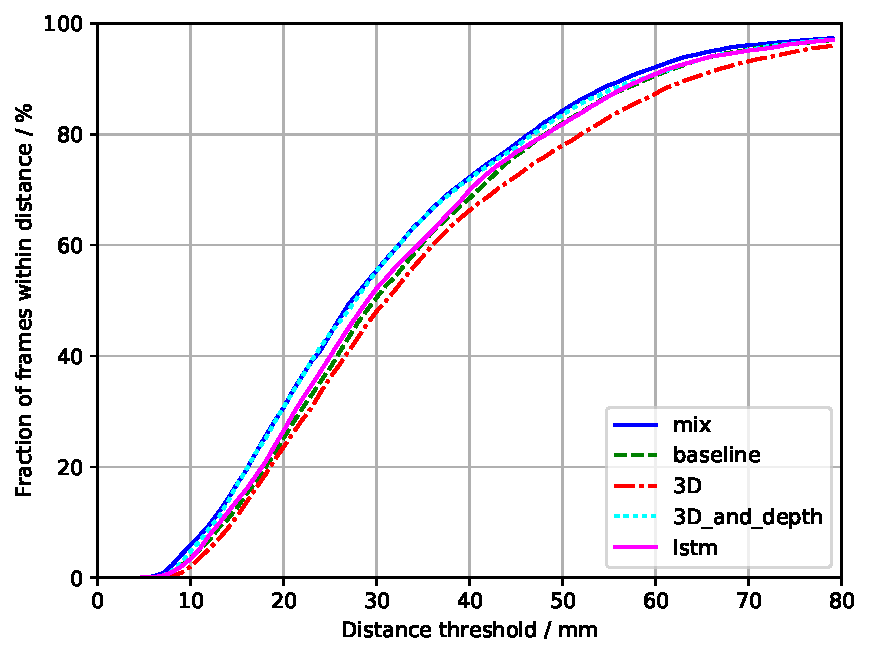
\includegraphics[width=1\linewidth]{src/experiment/eval/NYU/ablation/ablation_frameswithin.pdf}
        \end{minipage}
    }
    \\
    \subfloat[]{
        \label{fig:ablation joint mean NYU}
        \begin{minipage}[t]{200pt}
             \raggedleft
            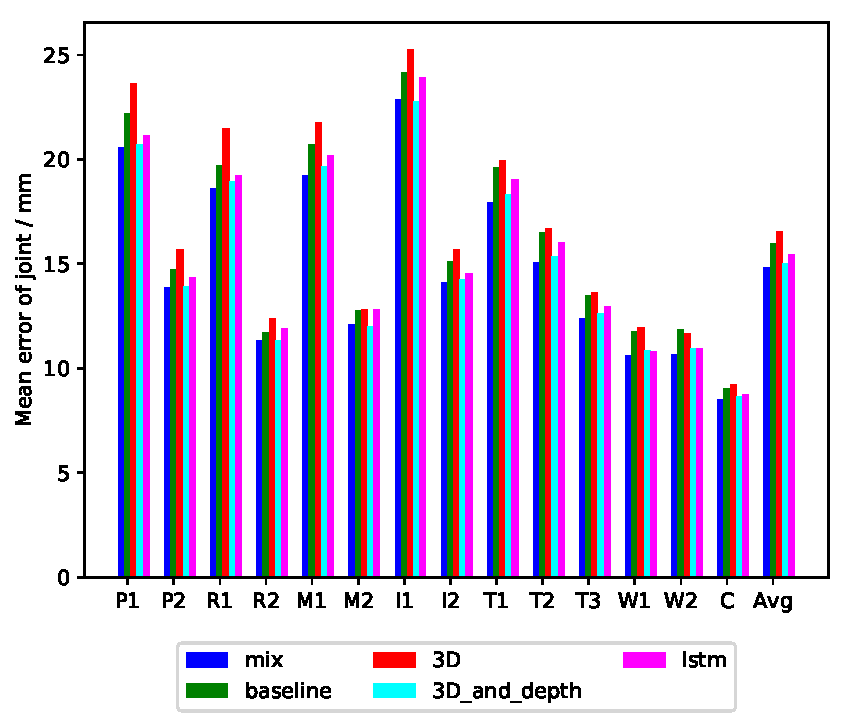
\includegraphics[width=1\linewidth]{src/experiment/eval/NYU/ablation/ablation_joint_mean.pdf}
        \end{minipage}
    }
    \caption{Performance of different part in our proposed network. Figure(a): proportion of good frames over
    different threshold for different part in our  proposed network (\textbf{3D} is the sliced 3D volumetric
    representation input branch in \emph{Spatial Network}, \textbf{Basic} is \emph{Basic Network}, \textbf{
    Spatial} is \emph{Spatial Network}, \textbf{Temporal} is \emph{Temporal Network}, and \textbf{Final}
    is our proposed \textbf{MSTN}). Figure(b): per-joint error distance for different parts. The palm and fingers
    are indexed as C: palm, T: thumb, I: index, M: middle, R: ring, P: pinky,W: wrist}
    \label{fig:result ablation}
\end{figure}

\begin{figure*}[t]\footnotesize
\centering
    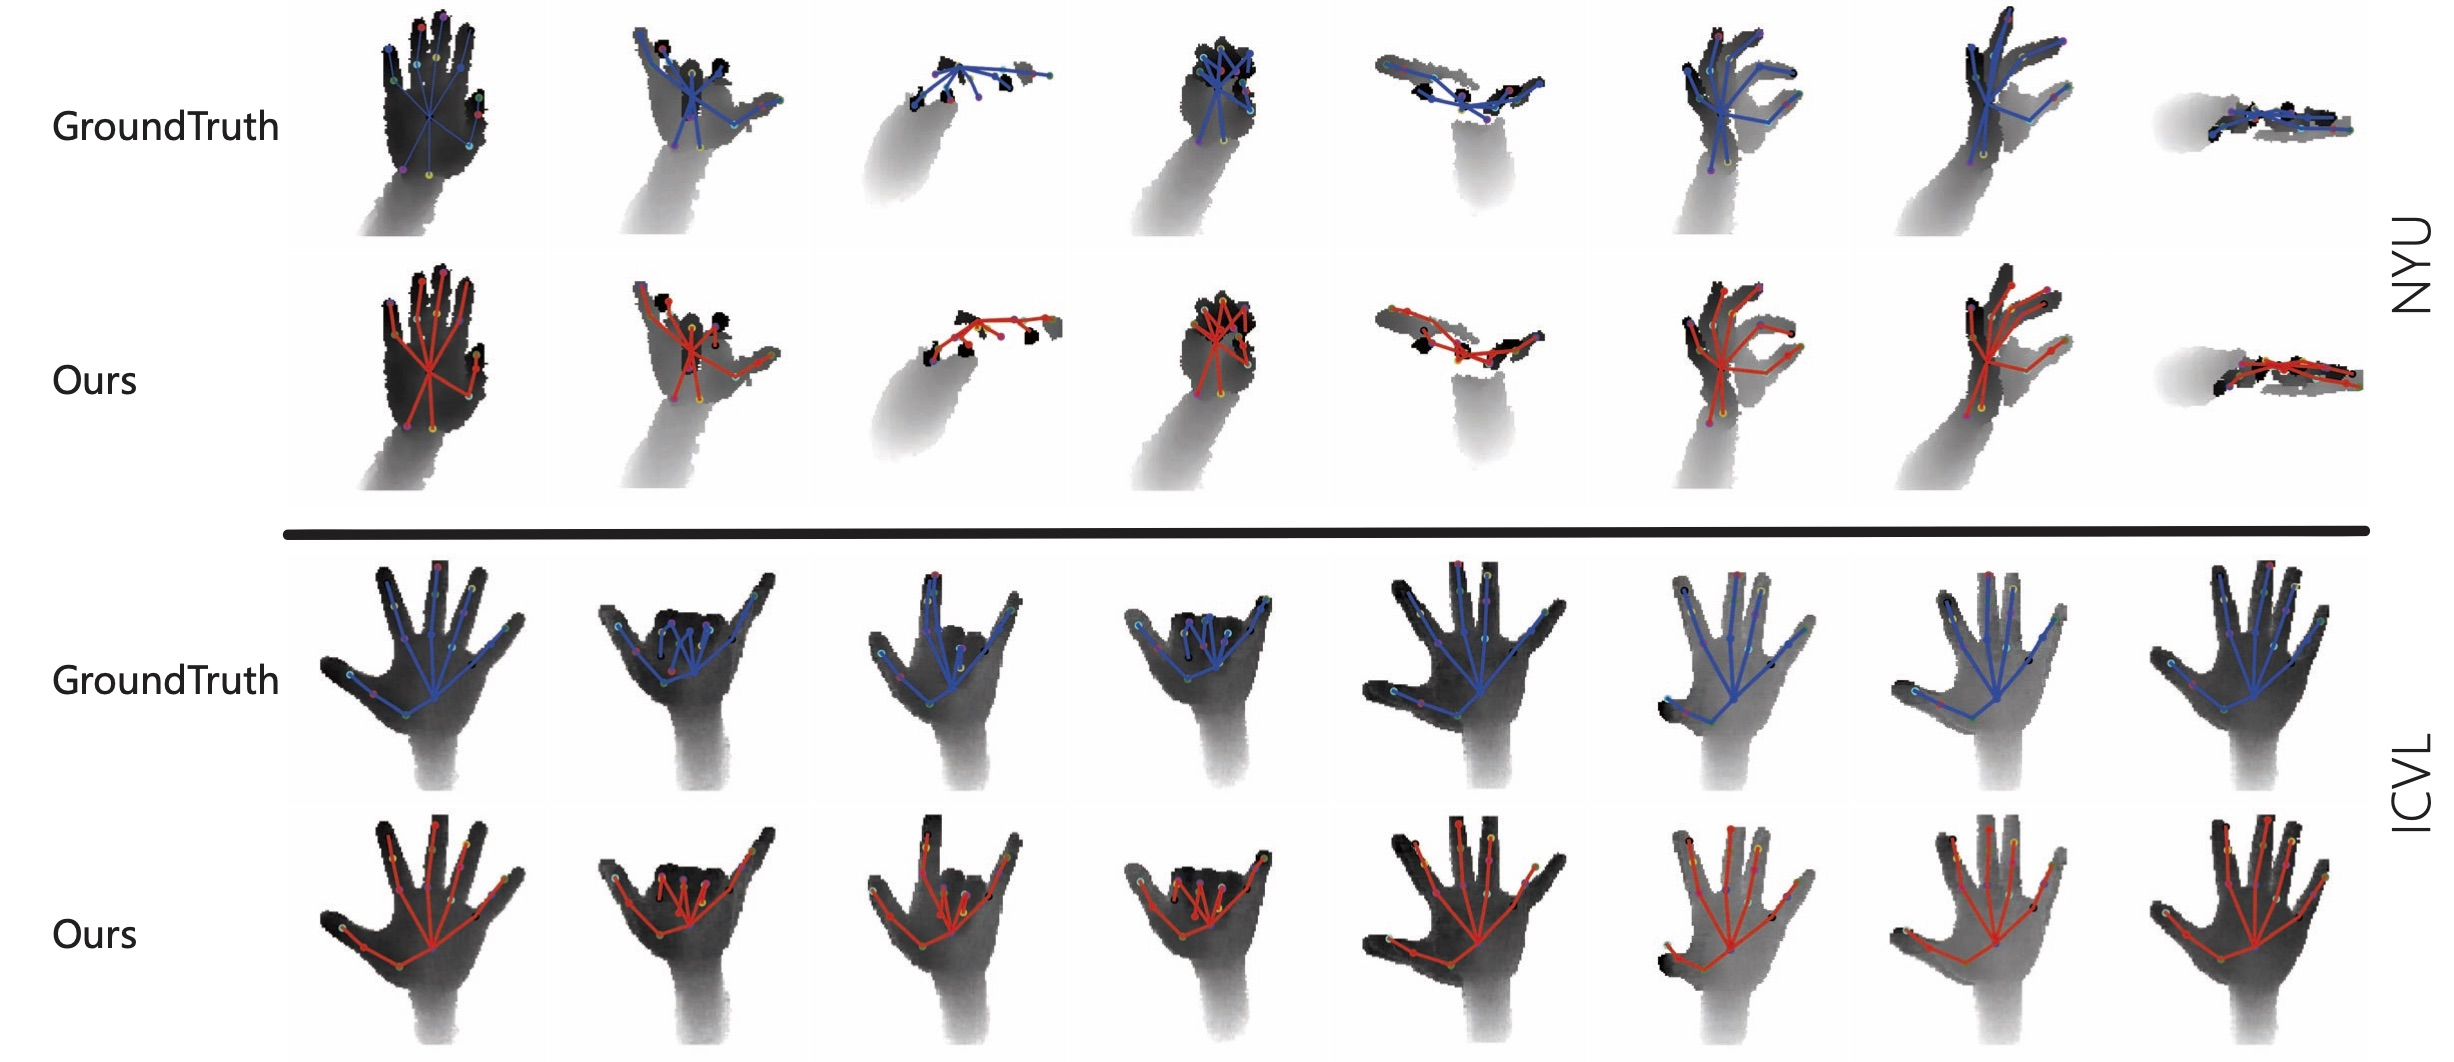
\includegraphics[width=1\linewidth]{src/experiment/qualitative_result.pdf}
    \caption{Qualitative results for NYU and ICVL dataset.}
\label{fig:qualitative result}
\end{figure*}

\section{Conclusion}\label{sec:conclusion}
In this paper, we present a hand pose estimation method called Mixture of Spatial-and-Temporal Network (\textbf{MSTN})
by keeping a watchful eye on accuracy, efficiency, robustness and stability. Our method extracts the features relate to
temporal coherence and spatial information by \emph{Temporal Network} and \emph{Spatial Network} respectively. By adopting
the Mixture of Experts framework, the predictions are weighted for final output. We evaluate \textbf{MSTN} on two publicly
available datasets and the experiments demonstrate that our method achieves the comparable results with several state-of-art
approaches.

\appendices


% use section* for acknowledgment
%\section*{Acknowledgment}


%The persons would like to thank...

\ifCLASSOPTIONcaptionsoff
  \newpage
\fi

\bibliography{wu}
\bibliographystyle{IEEEtran}

% that's all folks
\end{document}


